%%%%%%%%%% Subgroups %%%%%%%%%%
\chapter{\textsection\textsection Subgroups}

\section{\textsection Basic Definitions and Examples: Subgroups}

\begin{defn}
    A subset $H$ of a group $(G,\star)$ (i.e. $H \subseteq G$) is a \Emph{subgroup} if it satisfies the following properties:
    \begin{enumerate}
        \item[S1] (\Emph{identity}) $e \in H$, where $e$ is the identity in $G$ (so $H \neq \emptyset$)
        \item[S2] (\Emph{closure}) If $h_1,h_2 \in H$, then $h_1\star h_2 \in H$.
        \item[S3] (\Emph{inverses}) Of $h \in H$, then $h^{-1} \in H$.
    \end{enumerate}
    Thus, the group $(H,\star\vert_{H})$ makes sense. We denote this by $H \leq G$, to say $H$ is a subgroup of $G$ ($\star$ is understood from context)
\end{defn}

\begin{eg}
    \leavevmode
    \begin{enumerate}
        \item $\{e\} \leq G$ and $G \leq G$, for any group $G$. These subgroups are called the \Emph{trivial subgroups of $G$}.
        \item $\Z\leq \R$ with addition
        \item $l\Z := \{ln:n \in \Z\}\subset \Z$, where $l$ is fixed in $\Z$. $l\Z \leq \Z$. Indeed \begin{enumerate}
            \item[S1] $0 = l\cdot 0 \in l\Z$
            \item[S2] $ln+lm = l(n+m) \in l\Z$
            \item[S3] $ln + l(-n) = l(n+(-n)) = l\cdot 0 = 0$, so $-(ln) \in l\Z$.
        \end{enumerate}
        \item $SL_n(\R) := \{A \in Mat_n(\R):\det(A) = 1\} \leq \GL_2(\R)$ is a subgroup called the \Emph{special linear group} of degree $n$.
        \begin{proof}
            (Left to the reader)
        \end{proof}
        \item Let $S^1 := \{z \in \C:|z| = 1\}$, then $S^1 \leq \C\backslash\{0\} = \C^{\times}$, where the operation is multiplication. $S^1$ is called the \Emph{circle group}
    \end{enumerate}
\end{eg}


\begin{prop}
    If $H_1 \leq G$, $H_2 \leq G$ are subgroups of $G$, then $H = H_1 \cap H_2 \leq G$ is a subgroup.
    \begin{proof}
        (Left to the reader)
    \end{proof}
\end{prop}

\begin{cor}
    Let $\{H_{\alpha}\}_{\alpha \in J}$ be a collection of subgroups of a group $G$, where $J$ is an indexing set (possible infinite). Then \begin{equation}
        \bigcap_{\alpha \in J}H_{\alpha} \leq G
    \end{equation}
    \begin{proof}
        (Left to the reader)
    \end{proof}
\end{cor}

\subsection{\textsection Center}

\begin{defn}
    Let $(G,\star)$ be a group and let $g \in G$. The \Emph{centralizer} of $g \in G$ is \begin{equation}
        Z(g) := \{x \in G: \underbrace{x\star g = g \star x}_{x\text{ and }g\text{ commute}}\}
    \end{equation}
\end{defn}

\begin{claim}
    For all $g \in G$, for a group $(G,\star)$, $Z(g) \leq G$ is a subgroup of $G$.
    \begin{proof}
        (Left to the reader)
    \end{proof}
\end{claim}

\begin{eg}
    \leavevmode
    \begin{enumerate}
        \item $Z(2) \leq (\Z,+)$, and actually $Z(2) = \Z$ as $\Z$ is abelian.
        \item $Z(I_2 + E_{2,2}) \leq \GL_2(\R)$, and in particular $$Z(I_2+E_{2,2}) = \left\{\begin{pmatrix} a & 0 \\ 0 & d \end{pmatrix} \in \GL_2(\R):ad \neq 0, ad\in \R\right\}$$
    \end{enumerate}
\end{eg}

\begin{defn}
    The \Emph{center} $Z(G)$ of the group $G$ is \begin{equation}
        Z(G) := \{x \in G:x\star g = g \star x \forall g \in G\}
    \end{equation}
\end{defn}

\begin{prop}
    $Z(G) = \bigcap_{g \in G} Z(g)$, so also $Z(G) \leq G$.
\end{prop}

\begin{xca}
    For $n \geq 2$, $Z(\GL_n(\R)) \{aI_n: a \in \R^{\times}\}$
\end{xca}

\begin{rmk}
    For any group $G$, $Z(G)$ is an \Emph{abelian} group.
\end{rmk}


\section{\textsection Cyclic Subgroups}


\begin{defn}
    Let $S \subset G$ a subset of a group $G$. Then the \Emph{subgroup of $G$ generated by $S$} is \begin{equation}
        \langle S\rangle := \bigcap\{H \in \mathcal{P}(G): S \subset H \leq G\}
    \end{equation}
    (The intersection of all the subgroups of $G$ containing $S$) which is the smallest subgroup of $G$ containing $S$.
    \begin{note}
        $S \subset G \leq G$, so $S \subset \langle S \rangle$ and $\langle S \rangle$ is well-defined. $\langle S \rangle$ is the smallest subgroup of $G$ containing $S$ with respect to set inclusion.
    \end{note}
\end{defn}

\begin{eg}
    $\langle \emptyset\rangle = \{e\}$ and $\langle G \rangle = G$ (trivial subgroups)
\end{eg}

\begin{prop}
    Let $g \in G$, then \begin{equation}
        \langle \{g\}\rangle = \{g^n:n \in \Z\}
    \end{equation}
    and we write $\langle g \rangle := \langle \{g\}\rangle$.
    \begin{proof}
        (Left to the reader)
    \end{proof}
\end{prop}

\begin{eg}
    \leavevmode
    \begin{enumerate}
        \item $\langle e \rangle = \{e\}$
        \item For $[2] \in \Z/3\Z$, the $\langle [2] \rangle = \{[2], [1], [0]\} = \Z/3\Z$.
        \item For $l \in \Z$, $\langle l \rangle = \{nl:n\in\Z\}\leq \Z$. We write $l\Z := \langle l \rangle$.
    \end{enumerate}
\end{eg}

\begin{defn}
    A group $K$ such that there exists $g \in K$ with $\langle g \rangle = K$ is called a \Emph{cyclic group}.
\end{defn}
\begin{enumerate}
    \item[$\drsh$] i.e$\rangle$ A group generated by single element is called \Emph{cyclic}.
\end{enumerate}


\begin{defn}
    Then, for all $g \in G$, $\langle g \rangle \leq G$ is cyclic. The order of $|\langle g \rangle|$ of the group $\langle g \rangle$ is called the \Emph{order of $g$}, and denoted $o(g)$ (could be infinite!).
\end{defn}


\begin{eg}
    \leavevmode
    \begin{enumerate}
        \item For $1 \in \Z$, $o(1) = \infty$ given $\langle 1 \rangle = \Z$. Thus, $\Z$ is cyclic of infinite order.
        \begin{enumerate}
            \item[$\drsh$] \underline{Note:} The \underline{only} other generator of $\Z$ is $-1$.
            \begin{enumerate}
                \item[$\drsh$] For $2 \in \Z$ does not generate $\Z$ because $\langle 2 \rangle = 2\Z \subsetneq \Z$ 
            \end{enumerate}
        \end{enumerate}
        \item For $n \in \Z_{>0}$, $[1]_n \in \Z/n\Z$, $o([1]_n) = n$ given $$\langle [1]_n\rangle = \{k[1]_n:k \in \Z\} = \Z/n\Z$$
        Thus $\Z/n|Z$ is a cyclic group of order $n$.
        \item For any group $G$, $o(e) = 1$ where $e$ is the identity of $G$.
        \item $\Q^{\times} = (\Q\backslash\{0\},\cdot)$ is not cyclic.
        \begin{proof}
            Assume $\Q^{\times} = \langle \frac{a}{b}\rangle$, then take $p$ relatively prime to $a$ and to $p$. Then $p \notin \left\{\left(\frac{a}{b}\right)^n: n \in \Z\right\}$, which contradicts the assumption and $\Q^{\times}$ is not cyclic.
        \end{proof}
    \end{enumerate}
\end{eg}


\begin{rmk}
    A cyclic group is abelian.
    \begin{proof}
        (Left to the reader)
    \end{proof}
\end{rmk}

\begin{cor}
    If a group is non-abelian it cannot be cyclic.
    \begin{proof}
        Contrapositive of the previous statement.
    \end{proof}
\end{cor}
\begin{enumerate}
    \item[$\drsh$] $\GL_n(\R)$, $n \geq 2$, and $S_m$, $m \geq 3$, are not cyclic as they are non-abelian. 
\end{enumerate}


$\Z$ is cyclic and properties of $\Z$ will have consequences for all cyclic groups (through isomorphisms).

\begin{thm}
    Every subgroup $H$ of $(\Z,+)$ is of the form $n\Z = \langle n \rangle$ for some $n \in \Z$.
    \begin{proof}
        (Left to the reader)
    \end{proof}
\end{thm}

\begin{cor}[GCD]
    Let $a,b \in \Z$ and define \begin{equation}
        a\Z + b\Z := \{an + bm: n,m \in \Z\} \subset \Z
    \end{equation}
    $a\Z+b\Z$ is a subgroup of $(\Z,+)$ generated by $\{a,b\}$. Then, by the previous theorem $a\Z + b\Z = d\Z$ for some $d \in \Z$, and if $(a,b) \neq (0,0)$, we have that $d = \gcd(a,b)$. We choose $d > 0$ to maintain uniqueness.
    \begin{proof}
        (Left to the reader)
    \end{proof}
\end{cor}

\begin{cor}
    Suppose $a\Z + b\Z = d\Z$, $(a,b) \neq (0,0)$, so $d \neq 0$. Then \begin{enumerate}
        \item $d\;\vert\;a$ and $d\;\vert\;b$.
        \item If $e \;\vert\;a$ and $e\;\vert\;b$, then $e \;\vert\;d$.
        \item There exist $x,y \in \Z$ such that $d = ax + by$.
    \end{enumerate}
\end{cor}

\begin{prop}
    Take the cyclic subgroup $\langle g \rangle \leq G$ of $G$. Then define \begin{equation}
        S_g := \{k \in \Z: g^k = e\}\subset \Z
    \end{equation}
    It follows that \begin{enumerate}
        \item $S_g \leq \Z$ is a subgroup for all $g \in G$.
        \item For $r,s \in \Z$, $g^r = g^s$ if and only if $r-s \in S_g$.
        \item If $S_g \neq \{0\}$, then $S_g = n\Z$ for some $n >0$, and \begin{equation}
            \langle g \rangle = \{e,g,g^2,...,g^{n-1}\}
        \end{equation}
        with $o(g) =n$.
        \item $S_g = \{0\}$ if and only if $o(g) = \infty$, in which case $g^m = g^n$ if an only if $m = n$.
        \item The order of $g^l$ is $\frac{n}{\gcd(l,n)}$ if $o(g) = n$.
    \end{enumerate}
\end{prop}
\begin{proof}
    (Left to the reader)
\end{proof}

\begin{rmk}
    If $o(g) = \infty$, $g^r = g^s$ if and only if $r = s$. If $o(g) = n < \infty$, $g^r = g^s$ if and only if $r \equiv s \mod n$.
    \begin{enumerate}
        \item[$\drsh$] $o(g)$ is the smallest integer $n > 0$ such that $g^n = e$. (If $\cancel{\exists}n > 0$ such that $g^n = e$, then $o(g) = \infty$) 
    \end{enumerate}
\end{rmk}

\begin{cor}
    For $g \in G$, $g^l$ is a generator of $\langle g \rangle$ if and only if $\gcd(l,n) = 1$, where $n = o(g)$.
\end{cor}
\begin{enumerate}
    \item[$\drsh$] If $o(g) = \infty$ then $\langle g^l \rangle = \langle g \rangle$ if and only if $l \in \{1,-1\}$
\end{enumerate}
\begin{proof}
    (Left to the reader)
\end{proof}

\begin{thm}
    Every subgroup of a cyclic group is itself cyclic.
    \begin{proof}
        (Left to the reader)
    \end{proof}
\end{thm}

\begin{eg}
    \leavevmode
    \begin{enumerate}
        \item For $2 \in (
        \Z,+)$, $o(2) = \infty$, so $\langle 2 \rangle = 2\Z$, and $|2\Z| = \infty$.
        \item For $[2] \in \Z/3\Z$, $o([2]) = 3$, so $\langle [2]\rangle = \Z/3\Z$. Indeed, $\langle [1]\rangle = \Z/3\Z$, so $$o([2]) = o(2[1]) = \frac{o([1])}{\gcd(o([1]),2)} = \frac{3}{\gcd(3,2)} = 3$$
        \item For $[2] \in \Z/4\Z$, $o([2]) = 2$, so $\langle [2] \rangle < \Z/4\Z$ is a proper subgroup.
    \end{enumerate}
\end{eg}


\begin{cor}
        Let $G = \langle g \rangle$ be cyclic. Then every subgroup of $G$ is cyclic.
\end{cor}
\begin{proof}
        Consider the epimorphism \begin{equation}
                \map{\Z\xrightarrow{\phi_g}G}{n\mapsto g^n}
        \end{equation}
        Let $H \subseteq G$. Then $\phi^{-1}_g(H) = H' \subseteq \Z$ because of the properties of the inverse images of subgroups under group homomorphisms. Thus since $\phi_g$ is cyclic, $\phi_g(H') = H$, so $H$ is the image of a subgroup $H'$ of $\Z$. But, all subgroups of $\Z$ are cyclic. Thus $\phi_g(H')$ is cyclic since it is the image of a cyclic subgroup under a group homomorphism.
\end{proof}


\begin{thm}
        If $G$ is a cyclic group of order $n < +\infty$, then the order of every subgroup $H$ of $G$ divides $n$. Moreover, for every divisor $q$ of $n$, there exists a unique subgroup of $G$ of order $q$.
\end{thm}
\begin{proof}
        Let $G = \langle g \rangle$, $H \subseteq G$, and $o(g) = n$. By the previous corollary $H = \langle g^l \rangle$ for some $l \geq 0$. It follows that $|H| = \frac{n}{\gcd(n,l)}$. Thus, $$\frac{n}{\gcd(n,l)} = |H|\;\vert\;|G| = n$$ Suppose $|H| = |H'| (=\langle g^{l'}\rangle)$, so $\gcd(l,n) = \gcd(l',n)$. Note that $o(g^{\gcd(l,n)}) = \frac{n}{\gcd(n,\gcd(l,n))} = \frac{n}{\gcd(n,l)} = o(g^l)$ and since $\gcd(l,n)\;\vert\;l$ $g^l \in \langle g^{\gcd(l,n)}\rangle$. Hence, we have that \begin{equation}
                H = \langle g^l \rangle = \langle g^{\gcd(l,n)} \rangle = \langle g^{\gcd(l',n)} \rangle = \langle g^{l'} \rangle = H'
        \end{equation}
        Thus we have uniqueness, and that the order of any subgroup must divide that of the group. For existence, suppose $n = qr$ for some integer $r$. Then $H = \langle g^r\rangle$ is a subgroup of order $$|H| = o(g^r) = \frac{n}{\gcd(n,r)} = \frac{qr}{r} = q$$ satisfying existence.
\end{proof}



\section{\textsection Dihedral Groups}

\begin{claim}
    If $S$ is a non-empty subset of $G$, then \begin{equation}
        \langle S\rangle = \{s_1^{k_1}\star s_2^{k_2} \star ... \star s_m^{k_m}: m\geq 1, s_1,s_2,...,s_m \in S,k_1,k_2,...,k_m\in\Z\}
    \end{equation}
    Or, equivalently \begin{equation}
        \langle S\rangle = \{r_1^{\alpha_1}\star r_2^{\alpha_2} \star ... \star r_n^{\alpha_n}: n\geq 1, r_1,r_2,...,r_n \in S,\alpha_1,\alpha_2,...,\alpha_n\in\{1,-1\}\}
    \end{equation}
\end{claim}

\begin{rmk}
    The $s_i$'s (and $r_i$'s) in these two descriptions need not be distinct. This is a generalization of the description of $\langle g \rangle$. This is by no means a unique way to write elements of $\langle S\rangle$.
\end{rmk}

\begin{eg}
    For $S = \{a,b\}$, \begin{enumerate}
        \item If $a \star b = b \star a$, for all $m \geq 1$, \begin{equation}
            s_1^{k_1}\star s_2^{k_2} \star ... \star s_m^{k_m} = a^k \star b^l
        \end{equation}
        \item In additive notation we get $a^k \star b^l = ka + lb$, so $\langle \{a,b\}\rangle = \Z a + \Z b$. (In general this need not be cyclic)
    \end{enumerate}
\end{eg}

\begin{rmk}
    If we don't assume $a \star b = b \star a$, then we cannot simplify a general element to the form $a^k \star b^l$ in $\langle S \rangle$.
\end{rmk}


\begin{defn}
    A polygon $X$ is \Emph{regular} if it is \Emph{equiangular} (all angles are equal in measure) and \Emph{equilateral} (all sides have the same length).
\end{defn}
\begin{enumerate}
    \item[$\drsh$] \begin{note}
        The vertices of such a figure (if it is convex) can always be drawn on a circle called the \Emph{circumcircle}.
    \end{note} 
\end{enumerate}

\begin{eg}
    \leavevmode
    \begin{enumerate}
        \item $3$-sides $=$ equilateral triangle: \begin{center}
            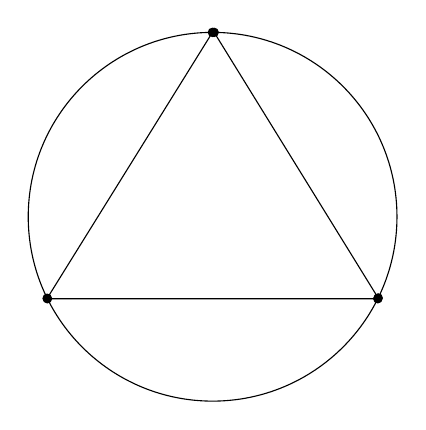
\begin{tikzpicture}[x=0.75pt,y=0.75pt,yscale=-1,xscale=1]
            %uncomment if require: \path (0,300); %set diagram left start at 0, and has height of 300
            
            %Shape: Circle [id:dp6369909468365647] 
            \draw   (66.67,160.5) .. controls (66.67,111.44) and (106.44,71.67) .. (155.5,71.67) .. controls (204.56,71.67) and (244.33,111.44) .. (244.33,160.5) .. controls (244.33,209.56) and (204.56,249.33) .. (155.5,249.33) .. controls (106.44,249.33) and (66.67,209.56) .. (66.67,160.5) -- cycle ;
            %Shape: Triangle [id:dp2358003807310185] 
            \draw   (155.83,71) -- (235.5,200) -- (75.67,200) -- cycle ;
            
            
            
            \draw [fill={rgb, 255:red, 3; green, 3; blue, 3 }  ,fill opacity=1 ]  (156.25, 71.67) circle [x radius= 2, y radius= 2]   ;
            \draw [fill={rgb, 255:red, 3; green, 3; blue, 3 }  ,fill opacity=1 ]  (235.27, 199.63) circle [x radius= 2, y radius= 2]   ;
            \draw [fill={rgb, 255:red, 3; green, 3; blue, 3 }  ,fill opacity=1 ]  (235.09, 200) circle [x radius= 2, y radius= 2]   ;
            \draw [fill={rgb, 255:red, 3; green, 3; blue, 3 }  ,fill opacity=1 ]  (75.91, 200) circle [x radius= 2, y radius= 2]   ;
            \draw [fill={rgb, 255:red, 3; green, 3; blue, 3 }  ,fill opacity=1 ]  (155.42, 71.67) circle [x radius= 2, y radius= 2]   ;
            \draw [fill={rgb, 255:red, 3; green, 3; blue, 3 }  ,fill opacity=1 ]  (75.8, 199.78) circle [x radius= 2, y radius= 2]   ;
            \end{tikzpicture}
        \end{center}
        \item $4$-sides $=$ square 
        \begin{center}
            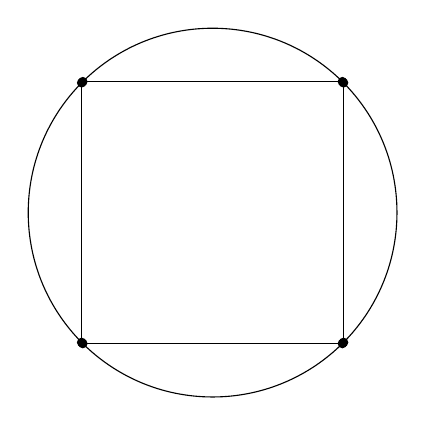
\begin{tikzpicture}[x=0.75pt,y=0.75pt,yscale=-1,xscale=1]
            %uncomment if require: \path (0,300); %set diagram left start at 0, and has height of 300
            
            %Shape: Circle [id:dp6369909468365647] 
            \draw   (66.67,160.5) .. controls (66.67,111.44) and (106.44,71.67) .. (155.5,71.67) .. controls (204.56,71.67) and (244.33,111.44) .. (244.33,160.5) .. controls (244.33,209.56) and (204.56,249.33) .. (155.5,249.33) .. controls (106.44,249.33) and (66.67,209.56) .. (66.67,160.5) -- cycle ;
            %Shape: Square [id:dp9411752355047514] 
            \draw   (92.4,97.4) -- (218.6,97.4) -- (218.6,223.6) -- (92.4,223.6) -- cycle ;
            
            
            
            \draw [fill={rgb, 255:red, 3; green, 3; blue, 3 }  ,fill opacity=1 ]  (92.97, 97.4) circle [x radius= 2, y radius= 2]   ;
            \draw [fill={rgb, 255:red, 3; green, 3; blue, 3 }  ,fill opacity=1 ]  (218.03, 97.4) circle [x radius= 2, y radius= 2]   ;
            \draw [fill={rgb, 255:red, 3; green, 3; blue, 3 }  ,fill opacity=1 ]  (218.6, 97.97) circle [x radius= 2, y radius= 2]   ;
            \draw [fill={rgb, 255:red, 3; green, 3; blue, 3 }  ,fill opacity=1 ]  (218.6, 223.03) circle [x radius= 2, y radius= 2]   ;
            \draw [fill={rgb, 255:red, 3; green, 3; blue, 3 }  ,fill opacity=1 ]  (218.03, 223.6) circle [x radius= 2, y radius= 2]   ;
            \draw [fill={rgb, 255:red, 3; green, 3; blue, 3 }  ,fill opacity=1 ]  (92.97, 223.6) circle [x radius= 2, y radius= 2]   ;
            \draw [fill={rgb, 255:red, 3; green, 3; blue, 3 }  ,fill opacity=1 ]  (92.4, 97.97) circle [x radius= 2, y radius= 2]   ;
            \draw [fill={rgb, 255:red, 3; green, 3; blue, 3 }  ,fill opacity=1 ]  (92.4, 223.03) circle [x radius= 2, y radius= 2]   ;
            \end{tikzpicture}
        \end{center}
        \item $5$-sides $=$ pentagon
        \begin{center}
            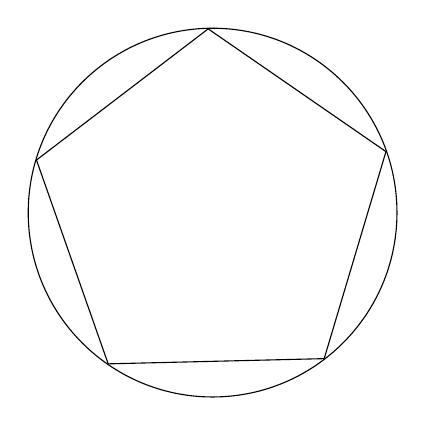
\begin{tikzpicture}[x=0.75pt,y=0.75pt,yscale=-1,xscale=1]
            %uncomment if require: \path (0,300); %set diagram left start at 0, and has height of 300
            
            %Shape: Circle [id:dp6369909468365647] 
            \draw   (66.67,160.5) .. controls (66.67,111.44) and (106.44,71.67) .. (155.5,71.67) .. controls (204.56,71.67) and (244.33,111.44) .. (244.33,160.5) .. controls (244.33,209.56) and (204.56,249.33) .. (155.5,249.33) .. controls (106.44,249.33) and (66.67,209.56) .. (66.67,160.5) -- cycle ;
            %Shape: Regular Polygon [id:dp6960584174528508] 
            \draw   (239.03,131.12) -- (209.26,230.86) -- (105.19,233.37) -- (70.65,135.17) -- (153.37,71.98) -- cycle ;
            
            
            
            
            \end{tikzpicture}
        \end{center}
        \item $n$-sides $=$ regular convex $n$-gon
        \begin{center}
            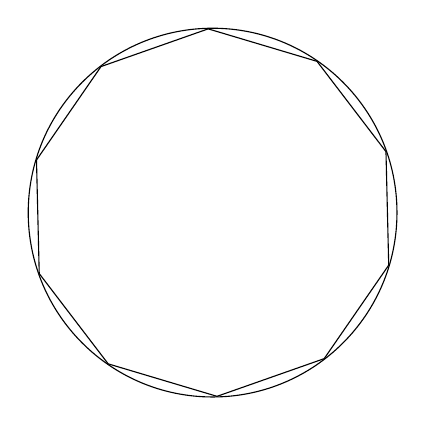
\begin{tikzpicture}[x=0.75pt,y=0.75pt,yscale=-1,xscale=1]
            %uncomment if require: \path (0,300); %set diagram left start at 0, and has height of 300
            
            %Shape: Circle [id:dp6369909468365647] 
            \draw   (66.67,160.5) .. controls (66.67,111.44) and (106.44,71.67) .. (155.5,71.67) .. controls (204.56,71.67) and (244.33,111.44) .. (244.33,160.5) .. controls (244.33,209.56) and (204.56,249.33) .. (155.5,249.33) .. controls (106.44,249.33) and (66.67,209.56) .. (66.67,160.5) -- cycle ;
            %Shape: Regular Polygon [id:dp6960584174528508] 
            \draw   (239.03,131.12) -- (240.35,185.83) -- (209.26,230.86) -- (157.63,249.02) -- (105.19,233.37) -- (71.97,189.88) -- (70.65,135.17) -- (101.74,90.14) -- (153.37,71.98) -- (205.81,87.63) -- cycle ;
            
            
            
            
            \end{tikzpicture}
        \end{center}
    \end{enumerate}
\end{eg}


\begin{defn}
    Let $n \geq 3$. The \Emph{dihedral group} $D_n$ is the \Emph{symmetry group} of the regular convex $n$-gon. Consider the following maps $\R^2 \rightarrow \R^2$:\begin{enumerate}
        \item For all $\alpha \in \R$, $\phi_{\alpha}$ is the rotation about the origin of $|R^2$ of angle $\alpha$ radians.
        \item For all $\alpha \in \R$, $\psi_{\alpha}$ is the reflection with respect to a line $l_{\alpha}$ going through the origin and forming an angle $\alpha$ radians with the $x$-axis:
        \begin{center}
            \begin{tikzpicture}[x=0.75pt,y=0.75pt,yscale=-1,xscale=1]
            %uncomment if require: \path (0,300); %set diagram left start at 0, and has height of 300
            
            \draw   (-1,170.8) -- (277.83,170.8)(138.42,89.2) -- (138.42,252.4) ;
            %Straight Lines [id:da1735016350905001] 
            \draw    (35.2,212.4) -- (245.35,125.56) ;
            \draw [shift={(247.2,124.8)}, rotate = 517.55] [color={rgb, 255:red, 0; green, 0; blue, 0 }  ][line width=0.75]    (10.93,-3.29) .. controls (6.95,-1.4) and (3.31,-0.3) .. (0,0) .. controls (3.31,0.3) and (6.95,1.4) .. (10.93,3.29)   ;
            %Shape: Arc [id:dp5422827964833219] 
            \draw  [draw opacity=0] (161.34,160.12) .. controls (163.99,162.87) and (165.6,166.46) .. (165.6,170.4) .. controls (165.6,170.48) and (165.6,170.55) .. (165.6,170.63) -- (148.4,170.4) -- cycle ; \draw   (161.34,160.12) .. controls (163.99,162.87) and (165.6,166.46) .. (165.6,170.4) .. controls (165.6,170.48) and (165.6,170.55) .. (165.6,170.63) ;
            \draw   (273.83,166.67) -- (278.17,170.58) -- (273.83,174.5) ;
            \draw   (134.42,93.1) -- (138.33,88.75) -- (142.26,93.07) ;
            
            % Text Node
            \draw (237.83,113.73) node [anchor=north west][inner sep=0.75pt]  [font=\tiny]  {$l_{\alpha }$};
            % Text Node
            \draw (169.5,160.4) node [anchor=north west][inner sep=0.75pt]  [font=\tiny]  {$\alpha $};
            
            
            \end{tikzpicture}
        \end{center}
    \end{enumerate}
\end{defn}

\begin{claim}
    For all $\alpha,\beta \in \R$, \begin{enumerate}
        \item $\phi_{\alpha} \circ \phi_{\beta} = \phi_{\alpha + \beta}$ (rotation) 
        \item $\psi_{\alpha} \circ \psi_{\beta} = \phi_{2(\alpha - \beta)}$ (rotation) 
        \item $\phi_{\alpha} \circ \psi_{\beta} = \psi_{\beta + \frac{1}{2}\alpha}$ (reflection) 
        \item $\psi_{\beta} \circ \phi_{\alpha} = \psi_{\beta - \frac{1}{2}\alpha}$ (reflection) 
    \end{enumerate}
    \begin{enumerate}
        \item[$\drsh$] (Where $\circ$ is the composition of maps $\R^2\rightarrow \R^2$). 
    \end{enumerate}
\end{claim}

\begin{note}
    This is \underline{not} commutative.
\end{note}


\begin{cor}
    The composition of maps induces a binary operation on the set of rigid motions and reflections about the origin, $\R^2\rightarrow \R^2$.
\end{cor}

\begin{prop}
    This set is a group with \begin{equation}
        \phi_{\alpha}^{-1} = \phi_{-\alpha}, \psi^{-1}_{\beta} = \psi_{\beta}, \;\text{and}\;\phi_0 = \id
    \end{equation}
    for all $\alpha,\beta \in \R$. Moreover, since $\circ$ is associative, it is indeed a group.
\end{prop}

\begin{defn}
    This group is called the \Emph{orthogonal group}, $O_2(\R)$.
\end{defn}

\begin{prop}
    Note that $O_2(\R) \leq \GL_2(\R)$ since the maps are linear. Indeed: \begin{equation}
        \phi_{\alpha} = \begin{bmatrix} \cos\alpha & -\sin\alpha \\ \sin\alpha & \cos\alpha \end{bmatrix}, \psi_{\alpha} = \begin{bmatrix} \cos2\alpha & \sin2\alpha \\ \sin2\alpha & -\cos2\alpha \end{bmatrix}, 
    \end{equation}
    in the standard basis of $\R^2$.
\end{prop}

\begin{defn}
    Let $N \geq 3$, the $n$-th \Emph{dihedral group $D_n$} is the subgroup of $O_2(\R)$ preserving a regular $n$-gon $X_n$ with a circumcircle centered at the origin of $\R^2$:\begin{equation}
        D_n := \{f \in O_2(\R): f(X_n) = X_n\}
    \end{equation}
\end{defn}

\begin{eg}
    For $n =6$ we have \begin{center}
        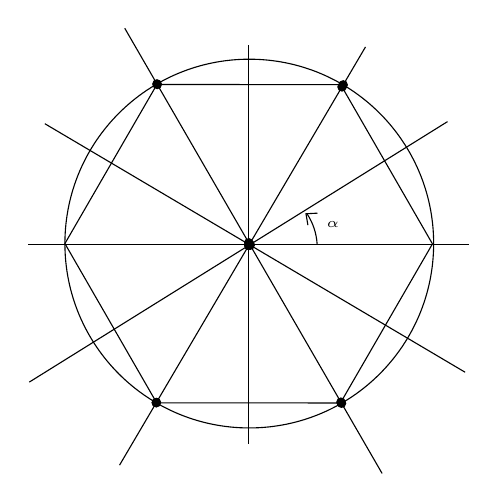
\begin{tikzpicture}[x=0.75pt,y=0.75pt,yscale=-1,xscale=1]
        %uncomment if require: \path (0,300); %set diagram left start at 0, and has height of 300
        
        %Shape: Circle [id:dp6369909468365647] 
        \draw   (66.67,160.5) .. controls (66.67,111.44) and (106.44,71.67) .. (155.5,71.67) .. controls (204.56,71.67) and (244.33,111.44) .. (244.33,160.5) .. controls (244.33,209.56) and (204.56,249.33) .. (155.5,249.33) .. controls (106.44,249.33) and (66.67,209.56) .. (66.67,160.5) -- cycle ;
        %Shape: Regular Polygon [id:dp6960584174528508] 
        \draw   (243.76,160.65) -- (199.42,237.3) -- (110.87,237.22) -- (66.67,160.5) -- (111.01,83.85) -- (199.55,83.93) -- cycle ;
        \draw   (49,161.13) -- (261.5,161.13)(155.25,65) -- (155.25,257.25) ;
        %Straight Lines [id:da00457972531911599] 
        \draw    (57,102.75) -- (259.5,222.5) ;
        %Straight Lines [id:da41124966975132526] 
        \draw    (49.5,227.25) -- (251,101.75) ;
        %Straight Lines [id:da32514486377192964] 
        \draw    (95.5,56.75) -- (219.5,271.25) ;
        %Straight Lines [id:da39830526708721803] 
        \draw    (211.5,65.75) -- (93,267.25) ;
        %Shape: Arc [id:dp7870194689907395] 
        \draw  [draw opacity=0] (183.31,146.13) .. controls (186.15,150.43) and (187.91,155.5) .. (188.2,160.96) -- (158.25,162.63) -- cycle ; \draw   (183.31,146.13) .. controls (186.15,150.43) and (187.91,155.5) .. (188.2,160.96) ;
        \draw   (183.75,151.63) -- (182.82,146.15) -- (188.37,145.84) ;
        
        % Text Node
        \draw (191.5,148.4) node [anchor=north west][inner sep=0.75pt]  [font=\tiny]  {$\alpha $};
        
        \draw [fill={rgb, 255:red, 3; green, 3; blue, 3 }  ,fill opacity=1 ]  (200.75, 84.04) circle [x radius= 2, y radius= 2]   ;
        \draw [fill={rgb, 255:red, 3; green, 3; blue, 3 }  ,fill opacity=1 ]  (110.67, 237.21) circle [x radius= 2, y radius= 2]   ;
        \draw [fill={rgb, 255:red, 3; green, 3; blue, 3 }  ,fill opacity=1 ]  (110.77, 237.04) circle [x radius= 2, y radius= 2]   ;
        \draw [fill={rgb, 255:red, 3; green, 3; blue, 3 }  ,fill opacity=1 ]  (200.17, 85.01) circle [x radius= 2, y radius= 2]   ;
        \draw [fill={rgb, 255:red, 3; green, 3; blue, 3 }  ,fill opacity=1 ]  (155.41, 161.13) circle [x radius= 2, y radius= 2]   ;
        \draw [fill={rgb, 255:red, 3; green, 3; blue, 3 }  ,fill opacity=1 ]  (155.25, 161.4) circle [x radius= 2, y radius= 2]   ;
        \draw [fill={rgb, 255:red, 3; green, 3; blue, 3 }  ,fill opacity=1 ]  (155.49, 160.99) circle [x radius= 2, y radius= 2]   ;
        \draw [fill={rgb, 255:red, 3; green, 3; blue, 3 }  ,fill opacity=1 ]  (155.26, 161.38) circle [x radius= 2, y radius= 2]   ;
        \draw [fill={rgb, 255:red, 3; green, 3; blue, 3 }  ,fill opacity=1 ]  (155.63, 160.76) circle [x radius= 2, y radius= 2]   ;
        \draw [fill={rgb, 255:red, 3; green, 3; blue, 3 }  ,fill opacity=1 ]  (111.02, 83.59) circle [x radius= 2, y radius= 2]   ;
        \draw [fill={rgb, 255:red, 3; green, 3; blue, 3 }  ,fill opacity=1 ]  (199.95, 237.43) circle [x radius= 2, y radius= 2]   ;
        \draw [fill={rgb, 255:red, 3; green, 3; blue, 3 }  ,fill opacity=1 ]  (199.65, 236.91) circle [x radius= 2, y radius= 2]   ;
        \draw [fill={rgb, 255:red, 3; green, 3; blue, 3 }  ,fill opacity=1 ]  (111.17, 83.85) circle [x radius= 2, y radius= 2]   ;
        \draw [fill={rgb, 255:red, 3; green, 3; blue, 3 }  ,fill opacity=1 ]  (155.84, 161.13) circle [x radius= 2, y radius= 2]   ;
        \draw [fill={rgb, 255:red, 3; green, 3; blue, 3 }  ,fill opacity=1 ]  (155.25, 160.11) circle [x radius= 2, y radius= 2]   ;
        \draw [fill={rgb, 255:red, 3; green, 3; blue, 3 }  ,fill opacity=1 ]  (155.9, 161.24) circle [x radius= 2, y radius= 2]   ;
        \draw [fill={rgb, 255:red, 3; green, 3; blue, 3 }  ,fill opacity=1 ]  (155.79, 161.05) circle [x radius= 2, y radius= 2]   ;
        \end{tikzpicture}
    \end{center}
    We have $6$-rotations $$\{\phi_{2\pi/6},\phi_{4\pi/6},\phi_{6\pi/6},\phi_{8\pi/6},\phi_{10\pi/6},\phi_{12\pi/6}\}$$ and $6$-reflections $$\{\psi_{\pi/6},\psi_{2\pi/6},\psi_{3\pi/6},\psi_{4\pi/6},\psi_{5\pi/6},\psi_{6\pi/6}\}$$
\end{eg}

\begin{cor}
    The order $|D_n|$ is $2n$ ($n$-rotations and $n$-reflections). In particular \begin{equation}
        D_n = \left\langle \left\{\phi_{2\pi/n},\psi_0\right\}\right\rangle
    \end{equation}
\end{cor}

\begin{rmk}
    $D_n \leq O_2(\R) \leq \GL_2(\R)$
\end{rmk}

\begin{defn}[Algebraic Description]
    $D_n$ is the group of order $2n$ generated by $2$ elements $x,y$ satisfying the \Emph{relations} \begin{equation}
        x^n = e, y^2 = e, yx = x^{-1}y
    \end{equation}
    (they imply $xyx = y$, and $x^kyx^k = y$ for all $k \in \Z$)
\end{defn}

\begin{rmk}
    The elements of $D_n$ are \begin{equation}
        D_n = \{e,x,x^2,...,x^{n-1},y,yx,yx^2,...,yx^{n-1}\}
    \end{equation}
    (This is closed under the multiplication using the relations above). In fact, $(x^ky)^{-1} = x^ky$ because $x^kyx^k = y$ implies $x^ky = yx^{-k}$.
\end{rmk}

\begin{rmk}
    Let $Y \subset X$. Then \begin{equation}
        \{f\in S_X:f(Y) = Y\} \leq S_X
    \end{equation}
    where $S_X$ is the group of symmetries of the set $X$.
\end{rmk}


\begin{rmk}
    For the orthogonal group $O_2(\R)$ we have the subgroup \begin{equation}
        D_n = \{f\in O_2(\R) \leq S_{\R^2}:f(X_n) = X_n\} \leq O_2(\R)
    \end{equation}
    which is the group of symmetries of the regular convex $n$-gon, $X_n$, denoted by $D_n$.
\end{rmk}

\section{\textsection Lattice Subgroups of a Group}

\begin{cons}
    Given a finite group $G$, we plot subgroups of $G$ with $\{e\}$ at the bottom and $G$ at the top. We draw paths upward between subgroups using the rule that an upward line connects a subgroup $A$ to a subgroup $B$ if and only if $A \leq B$, and there are no subgroups properly between $A$ and $B$.
\end{cons}

\begin{rmk}
    If $G \cong H$, then $G$ and $H$ have the same lattice structure. That is, group isomorphism induces a one-to-one correspondence between subgroups preserving containment.
\end{rmk}

\begin{eg}
    \leavevmode
    \begin{enumerate}
        \item For $G = \Z/n\Z$ the lattice of subgroups is the lattice of divisors of $\Z$. For instance: 
        \begin{figure}[H]
            \centering
            \begin{tikzcd}
                & \Z/12\Z & & \\
                \ip{3} \arrow[ur, dash] & & \ip{2} \arrow[ul, dash] & \\
                & & & \ip{4} \arrow[ul, dash] \\
                & \ip{6} \arrow[uul, dash] \arrow[uur, dash] & & \\
                & & \ip{12} = \{0\} \arrow[ul, dash] \arrow[uur, dash] &
            \end{tikzcd}
            \label{fig:Z12Lattice}
        \end{figure}
        and for a prime p:
        \begin{figure}[H]
            \centering
            \begin{tikzcd}
                \Z/p^n\Z = \ip{1} \\
                \ip{p} \arrow[u, dash] \\
                \ip{p^2} \arrow[u, dash] \\
                \vdots \arrow[u, dash] \\
                \ip{p^{n-1}} \arrow[u, dash] \\
                \ip{p^n} = \{0\} \arrow[u, dash] \\
            \end{tikzcd}
            \label{fig:ZpLattice}
        \end{figure}
        \item The Klien $4-$group, $V_4 = \langle a,b,c: a^2=b^2=c^2=1\rangle$:
        \begin{figure}[H]
            \centering
            \begin{tikzcd}
                &V_4& \\
                \ip{a} \arrow[ur, dash] & \ip{b} \arrow[u, dash] & \ip{c} \arrow[ul, dash] \\
                &1 \arrow[ul, dash] \arrow[u, dash] \arrow[ur, dash]& \\
            \end{tikzcd}
            \label{fig:V4Lattice}
        \end{figure}
        \item The symmetric group on 3-letters, $S_3$:
        \begin{figure}[H]
            \centering
            \begin{tikzcd}
                & & S_3 & \\
                & & & \ip{(1\;2\;3)} \arrow[ul, dash] \\
                \ip{(1\;2)} \arrow[uurr, dash]& \ip{(2\;3)} \arrow[uur, dash] & \ip{(1\;3)} \arrow[uu, dash] &  \\
                & & (1) \arrow[ull, dash] \arrow[ul, dash] \arrow[u, dash] \arrow[uur, dash] &
            \end{tikzcd}
            \label{fig:S3Lattice}
        \end{figure}
    \end{enumerate}
\end{eg}
